\documentclass[spanish]{article}

\usepackage{sectsty}
\usepackage{babel}
\usepackage{graphicx}
\usepackage{wrapfig}
\usepackage{booktabs}
\usepackage{longtable}

% Margins
\topmargin=-0.45in
\evensidemargin=0in
\oddsidemargin=0in
\textwidth=6.5in
\textheight=9.0in
\headsep=0.25in

\title{  }
\author{  }
\date{\today}

\begin{document}
\maketitle	
\pagebreak

% Optional TOC
\tableofcontents
\pagebreak

%--Paper--


\section{INCENDIOS HISTÓRICOS}

\subsection{Riba de Saelices}
El incendio de Guadalajara de 2005 fue un incendio forestal que asoló parte de la provincia de Guadalajara (Castilla-La Mancha) desde el 16 hasta el 20 de julio de 2005 y que se cobró la vida de once bomberos forestales de los equipos de extinción.1​ Su origen fue una barbacoa que unos excursionistas descuidaron en un merendero cercano a la cueva de los Casares en el municipio de Riba de Saelices. Ardieron 10 352,57 ha de monte arbolado, en su mayor parte masas de pino resinero, sabina mora y roble, 2380,16 ha de matorral y pasto, y 154,64 ha de superficie no forestal.2​ El incendio devastó 2400 ha de alto valor ecológico pertenecientes al parque natural del Alto Tajo. Hubo medio millar de desalojados, incluyendo poblaciones enteras como Ciruelos del Pinar y Tobillos, entre otras.3​


La gestión que del incendio tuvo el gobierno de Castilla-La Mancha fue duramente criticada desde distintos ámbitos alegando que no se enviaron los medios aéreos y terrestres necesarios durante las primeras horas.4​ Dichas críticas se basaban entre otras, en las grabaciones del 1125​ y a que solo se elevó el nivel de alerta y se solicitó ayuda al gobierno central cuando se conoció la trágica noticia de los once muertos, como reconoció el entonces vicepresidente de la Junta Máximo Díaz Cano.6​


El 17 de diciembre de 2005, cerca de 5000 personas según la policía, 10 000 según los organizadores, se manifestaron en Guadalajara para homenajear a los fallecidos y exigir responsabilidades.7​ 
\subsubsection{Origen y desarrollo del incendio}
En la mañana del sábado 16 de julio de 2005, un grupo de nueve excursionistas realizaron una visita a la cueva de los Casares con la intención posterior de preparar una barbacoa en el merendero que se encuentra en la margen izquierda del río Linares, a unos cien metros de la boca de la gruta.8​ Mientras el grueso del grupo visitaba la cueva guiados por el guarda Emilio Moreno, los otros tres integrantes prepararon un fuego en dos parrillas de obra situadas en el área recreativa y lo alimentaron con hierba seca, ramas y piñas que recogieron de los alrededores. Al finalizar la visita el guarda observó los fuegos y les advirtió que el uso de las barbacoas estaba autorizado pero que él lo desaconsejaba severamente debido al fuerte viento que soplaba en el lugar, las altas temperaturas —superiores a 33 °C— y la abundancia de rastrojos secos: «le dije a Marcelino que la podía liar por el día que hacía. Ni al más tonto de mi pueblo se le ocurre hacer una barbacoa en un día así, con un viento infernal y al lado de un rastrojo. Eso es de no tener conocimiento».9​ En torno a las 14:40 una pavesa o brasa cayó de la barbacoa situada más al sur, que estaba sin vigilancia, prendió en la hierba seca y el fuego se propagó rápidamente en dirección noreste, a través del bosque de ribera y campos de cereal hasta alcanzar una zona forestal formada por pino resinero.10​11​8​


El incendio, avivado por el fuerte viento, se volvió incontrolable y a media tarde obligó a la evacuación de quinientos vecinos de las localidades de Ciruelos del Pinar, Tobillos y Mazarete.12​ Medios terrestres combatieron el fuego durante toda la noche, que al amanecer del domingo 17 de julio presentaba dos frentes activos con dirección a Cobeta y Luzón, respectivamente. A lo largo del día se incorporaron más efectivos a la lucha contra el fuego que ya contaba con tres aviones de carga en tierra, dos hidroaviones —se incorporaron dos más a última hora de la tarde—, dos helicópteros, quince equipos de maquinaria pesada, dos BRIF, así como varios retenes de tierra y equipos del Consorcio provincial de extinción de incendios de Guadalajara.13​
Un helicóptero Kamov 32A del Ministerio de Medio Ambiente.


A lo largo del domingo 17 de julio los vecinos de Mazarete pudieron regresar a su localidad pero el incendio seguía activo en tres frentes: Mazarete-Anquela-Selas, Ciruelos del Pinar-Luzón-Santa María del Espino y otro, irregular, hasta Villarejo de Medina. El más preocupante era el que amenazaba Luzón y Santa María del Espino y a las 18:00 se ordenó la evacuación de ambas localidades. Las carreteras GU-951, entre Ciruelos del Pinar y Mazarete; la GU-944, entre Mazarete y Cobeta; y la GU-949, entre Mazarete y Ablanque estaban cortadas. La carretera CM-2107 estaba habilitada únicamente para el servicio de extinción de incendios.13​


A última hora de la tarde comenzaron a circular rumores sobre la muerte de varios miembros del retén de Cogolludo cercados por el fuego. A las 21:30 la Subdelegación del Gobierno en Guadalajara confirmó esos rumores y unas horas después se localizaron los cadáveres de once agentes forestales —diez hombres y una mujer— en la ladera de un barranco.14​ Solo sobrevivió uno de los miembros del retén que encontró refugio bajo el chorro de agua que caía del camión accidentado en el que había intentado huir de las llamas.15​


El lunes, 18 de julio, se recuperaron los cadáveres de los brigadistas y se controlaron los frentes que amenazaban a las poblaciones de Santa María del Espino, Luzón, Tobillos, Mazarete, Anquela del Ducado y Villarejo de Medina. El 20 de julio se lograron controlar todos los frentes del incendio que todavía permanecían activos
\subsubsection{El proceso judicial}
La fase de instrucción del proceso penal contra los responsables del incendio se tramitó en el Juzgado de Instrucción de Sigüenza. En un principio estuvieron imputados en él los nueve excursionistas y el guardia forestal de la zona, pero en el año 2007 se amplió la imputación a veinte personas más, entre las que estaban varios altos cargos de la Junta de Castilla-La Mancha, quienes demostraron ante el juez que su labor fue impecable.16​


El juicio se desarrolló en la Audiencia Provincial de Guadalajara entre los años 2009 y 2012 y finalizó con una sentencia en la que se condenó únicamente a uno de los excursionistas por un delito de incendio forestal cometido por imprudencia grave y le impuso una condena de dos años de prisión, una multa de 3650 € y una indemnización de 10 640 971,14 € a la Junta de Castilla-La Mancha en concepto de daños causados por el incendio.16​ Esta sentencia fue recurrida por el condenado y ratificada por el Tribunal Supremo en el año 2013.


\subsection{Horta de Sant Joan}
El incendio de Horta de Sant Joan se inició el 20 de julio de 2009 y afectó al parque natural de Els Ports, en Horta de Sant Joan (Tarragona). Las montañas de Els Ports forman un macizo de relieve muy complejo a caballo entre el sistema ibérico y el sistema mediterráneo. Están formadas por materiales calcáreos que determinan un relieve abrupto y roto por varias fallas, con importantes solapamientos. Orográficamente la zona del incendio tiene crestas con un elevado grado de inaccesibilidad, con barrancos y torrentes muy estrechos y fuertes pendientes. 
\subsubsection{Inicio de los incendios}
Pese a que en un primer momento se creía que el incendio había sido provocado por un rayo,1​ posteriormente se demostró que el incendio fue causado por dos jóvenes al encender una hoguera. Según la juez de Gandesa (Tarragona) que investigó el incendio forestal de Horta de Sant Joan, se utilizó un acelerador de combustión, como podrían ser las bombonas de camping gas que previamente habían comprado los autores del incendio. 
\subsubsection{Características meteorológicas en el momento del incendio}
La situación meteorológica en ese periodo era de altas temperaturas y bajas humedades relativas. A nivel local, se daban cambios de intensidad y dirección del viento. Además, se añadía la inestabilidad tormentosa, lo cual implicaba rachas de viento erráticas y repentinas.2​


El fuego estuvo situado entre las carreteras T-330, que se cortó al ser atravesada por las llamas sobre las 16:30 horas, y la T-334, al sur del municipio, en la zona de Les Capçades. Las llamas se habían ido acercando al municipio. Las tareas de extinción se pudieron ver facilitadas por la lluvia que empezó a caer a última hora de la tarde. Efectivos de la Comunidad Valenciana, de Aragón y de la Unidad Militar de Emergencias (UME) del Ministerio de Defensa apoyaron a los bomberos de la Generalidad de Cataluña. 
\subsubsection{Comportamiento del incendio y maniobras de extinción}
En el incendio se registraron dos focos secundarios. Las longitudes de las llamas en plena alineación llegaron hasta los 50 metros. Durante las noches del 20 al 21 de julio de 2009, las llamas llegaron a los 20 metros. El 21 de julio de 2009, el viento de componente aumentó en intensidad, con rachas muy fuertes, cosa que produjo que el fuego quedase fuera de la capacidad de extinción. El 22 de julio de 2009, se produjo un cambio en la situación meteorológica y se reavivó el fuego por una zona que ya había quedado controlada. El 24 de julio de 2009, a las 11 de la mañana, quedó controlado el fuego, el cual se daría por extinguido el 3 de agosto de 2009. 
\subsubsection{Consecuencias}
El incendio afectó a unas 1140 hectáreas de vegetación,3​ principalmente pino blanco. En las tareas de extinción del incendio, perdieron la vida 5 bomberos de entre 31 y 47 años mientras trabajaban en las tareas de extinción del fuego y uno de ellos resultó gravemente herido. Los seis operarios, que pertenecían al Grupo de Refuerzo de Actuaciones Forestales (GRAF) un grupo de bomberos profesionales especializados en incendios forestales, trabajaban en primera línea para frenar el avance del fuego cuando, alrededor de las cuatro de la tarde del 21 de julio de 2009, un súbito cambio de viento les sorprendió, según explicó el secretario general del interior, Joan Boada. Al parecer, aunque los efectivos se taparon con una manta ignífuga, murieron o quedaron muy malheridos. Los dos supervivientes fueron traslados al Hospital Valle de Hebrón de Barcelona.
\subsubsection{Consecuencias políticas y comisión de investigación}
La forma en que se gestionaron las tareas de extinción fue casi de inmediato sometida a evaluación política, lo cual provocó enfrentamientos entre el Gobierno catalán y el Ayuntamiento de Horta, que se expandieron a discusiones técnico-políticas entre CiU (partido que gobernaba en Horta y entonces en la oposición en el parlamento autonómico) y el gobierno autonómico tripartito (que estuvo en el poder hasta noviembre de 2010). Desde el 8 de febrero hasta el 18 de marzo de 2010, tuvo lugar una comisión parlamentaria, promulgada y aprobada con el voto favorable de un tercio de los parlamentarios (de los partidos en la oposición). En ella compareció población local y cargos políticos y técnicos con un papel relevante durante la extinción o bien un cierto conocimiento del territorio. Aunque la comisión sirvió para la recopilación de mucha información técnica, formal y política sobre la gestión de la extinción del incendio, sus objetivos no fueron valorados de forma homogénea: mientras que para algunas personas se trataba de «buscar responsabilidades políticas, porque decir que todo ha sido causado por circunstancias meteorológicas o técnicas no permite mejorar la organización» (representante de CiU en la Comisión Parlamentaria celebrada el 3 de febrero de 2010), otras consideraban que la comisión había sido creada para alimentar un «fuego político y mediático, cuyo nombre es “Elecciones 2010”» (bombero del GRAF en la Comisión Parlamentaria del 22 de febrero de 2010).4​ TV3 dedicó un documental del programa semanal "Sense Ficció" a los aspectos técnicos del incendio





\section{HELICÓPTEROS}

\subsection{Sokol}
\begin{wrapfigure}{R}{0.5\textwidth}
  \begin{center}
    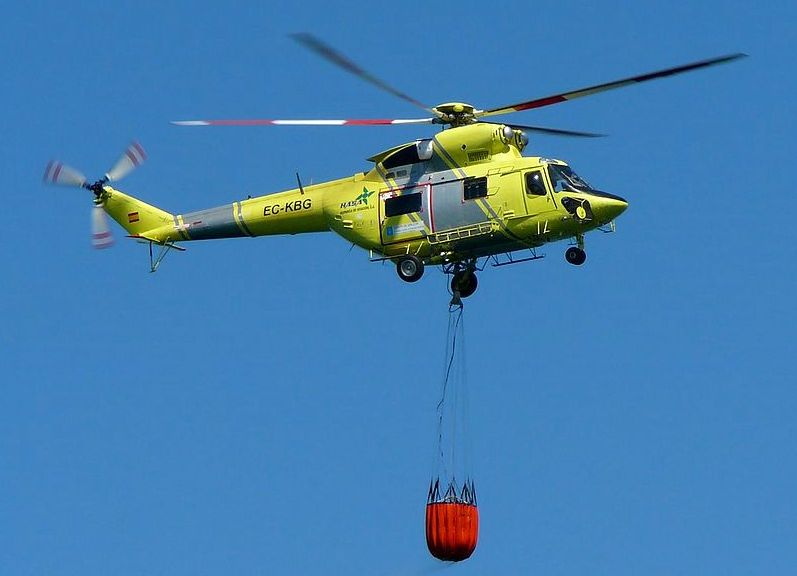
\includegraphics[width=0.35\textwidth]{images/sokol.jpg}
  \end{center}
  \caption{Ejemplo imagen a la derecha}
\end{wrapfigure}
El PZL W-3 Sokół (en polaco significa halcón) es un helicóptero utilitario medio de origen polaco. Se trata de un aparato bimotor de dos plazas que cuenta con un rotor principal de cuatro palas y otro de cola de tres palas. Tiene versiones diseñadas para misiones de transporte de personas y carga, también para asalto aéreo, búsqueda y rescate, SAR y de ataque. 
\subsubsection{Desarrollo}
El W-3 Sokol ('halcón') es el primer helicóptero totalmente diseñado y construido en serie en Polonia. En 1970, Polonia y la URSS firmaron un acuerdo de cooperación para la construcción y el desarrollo de un helicóptero polivalente. El proyecto fue iniciado por la empresa WSK PZL Świdnik en 1973 bajo la dirección de Stanisław Kamiński. En 1976 estuvo listo el primer prototipo y el Sokol hizo su primer vuelo el 16 de noviembre de 1979. Desde entonces ha sido certificado en Polonia, Rusia, EE. UU. y Alemania. Después de un programa de desarrollo bastante prolongado, la producción comenzó durante 1985 en cantidades limitadas. Las primeras ventas del Sokół multipropósito fueron a Polonia y al Bloque del Este antes de la caída del comunismo, lo que permitió a PZL Swidnik ampliar su base de ventas. Con la disolución del Pacto de Varsovia PZL se abrió a Occidente y en 1989 se inició la construcción de una nueva variante. Para ello desarrolló el mejorado Swidnik PZL Sokol W3A encaminado a lograr certificación occidental. La certificación bajo la norma FAR Pt 29 norteamericana se concedió en mayo de 1993, mientras que la certificación alemana fue concedida en diciembre de ese año. El 30 de julio de 1992 lanzó su primer vuelo la producción actual de la variante civil. También se exporta una versión militar.


La versión actual del PZL W-3A2, que recibió la aprobación de Polonia en el 7 de marzo de 2003, cuenta con un sistema electrónico de vuelo EFIS, es decir, un piloto automático de cuatro ejes que junto con el GPS realiza la ubicación y traza una ruta de vuelo de forma autónoma. Además, para las tareas de rescate y transporte, es posible emplear vuelo automático hasta el sitio.


El Sokol es un diseño y construcción convencional, con dos turboejes PZL-10W, que se basan en el PZL-10S versión con licencia de las turbohélices TVD-10B de diseño ruso que potencian el An-28 de construcción polaca también bajo licencia. Materiales compuestos son utilizados en las tres palas del rotor de cola y en las cuatro palas del rotor principal.


El Sokol se ofrece en una serie de variantes y es capaz de realizar un rango de misiones típicas de helicópteros, incluido el transporte de pasajeros, transporte VIP, de carga, EMS (servicios médicos de emergencia de algunos países), evacuación médica, extinción de incendios además de búsqueda y rescate.


La máquina es operada en su versión tanto civil como militar en Chequia, Alemania, España, Birmania, Chile ( Conaf Corporación Nacional Forestal), Polonia (Sily Powietrzne Rzeczypospolitej Polskiej), Portugal, Corea del Sur, Rusia y los Emiratos Árabes Unidos. Hasta 13 de septiembre de 2005 se han construido un total de 146 máquinas completas y cinco de las cabinas en ocho series del PZL W-3. 
\subsubsection{Historia operacional}
Desde 2003 cuatro PZL W-3WA fueron operados por el Grupo Independiente de Ataque Aéreo (Grupa Samodzielna Powietrzno-Szturmowa en polaco) de las fuerzas polacas en Irak. Uno de ellos (número de serie 360902) se estrelló en un accidente cerca de Kerbala, el 15 de diciembre de 2004. Tres soldados murieron y otros tres resultaron heridos.2​


El 3 de abril de 2015 en Nijar (Almería) aparece volcado una de las variantes de carga pintada de amarillo y matrícula EC-KIR, utilizada hasta el verano de 2014 en la lucha contra incendios. Las autoridades investigan cómo ha podido aparecer allí, en la zona no se ha localizado ni a pasajeros, carga o pilotos.


\subsection{Kamov}
\begin{wrapfigure}{r}{0.5\textwidth}
  \begin{center}
    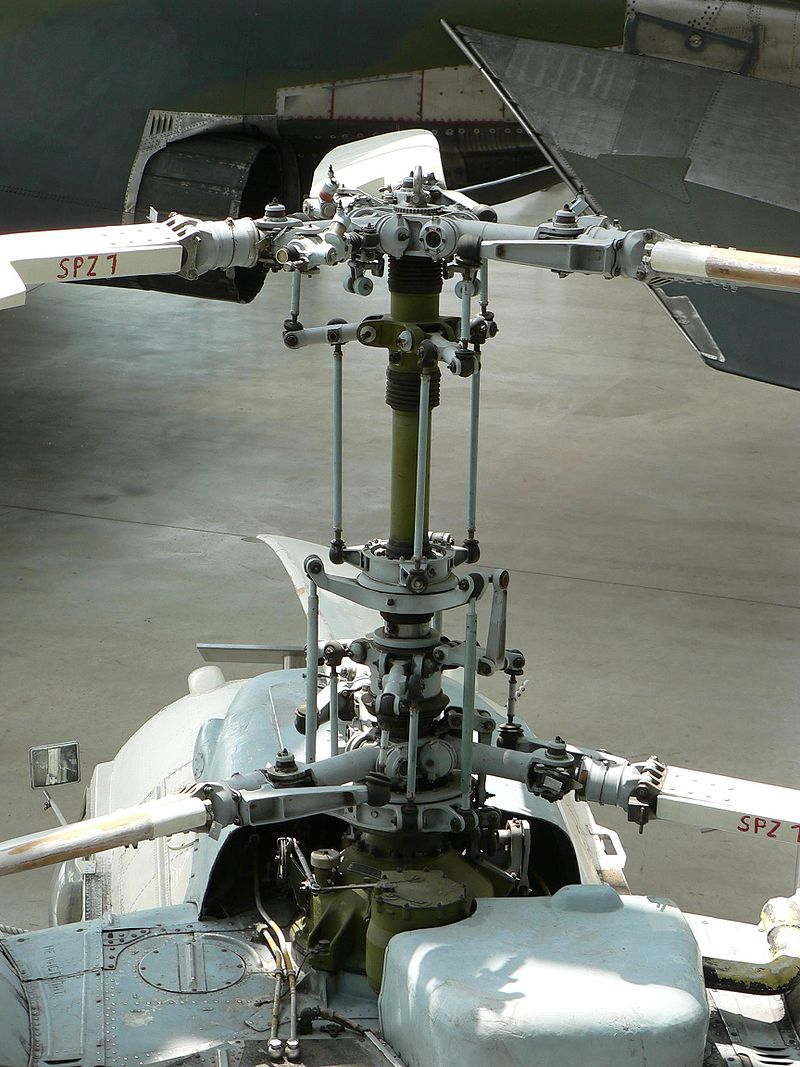
\includegraphics[width=0.28\textwidth]{images/kamov.jpg}
  \end{center}
  \caption{Ejemplo de imagen a la derecha no flotante}
\end{wrapfigure}
Kamov (en ruso: Камов) es un fabricante ruso de helicópteros, que ha heredado la fabricación de la antigua OKB-938 (en ruso: Особое Конструкторское Бюро), fundada en la Unión Soviética por Nikolái Kámov en el año 1948.


Kamov es una empresa especializada en la fabricación de helicópteros, que tienen como característica principal la de montar rotores coaxiales contrarrotativos.


En el año 2006 Mil se fusionó con Kamov y Rostvertol para formar la Corp. Oboronprom, la marca Kamov se mantendrá, pero se limitarán las nuevas líneas de productos.


Los rotores coaxiales cuentan con ciertas ventajas, entre ellas alta maniobrabilidad, fácil manejo y pequeñas dimensiones. Los helicópteros coaxiales son los de primer lugar en producción dentro del país y en el mundo, y se han convertido en el tipo de uso múltiple a bordo de helicópteros, caso del modelo Ka-15 (1957). Kamov es prácticamente la única empresa en el mundo que ha dominado los helicópteros con el esquema coaxial y a su vez ha implantado su producción a gran escala con aplicaciones prácticas, lo cual le ha permitido competir con éxito en el mercado frente a las principales compañías mundiales de helicópteros. 





\section{INCENDIOS POR PROVINCIAS}

\subsection{Teruel}
Los 10 incendios más grandes la provincia de Teruel son los siguientes:
\begin{longtable}{llr}
\toprule
FIREDATE & COMMUNE & sup \\
\midrule
\endfirsthead
\toprule
FIREDATE & COMMUNE & sup \\
\midrule
\endhead
\midrule
\multicolumn{3}{r}{Continued on next page} \\
\midrule
\endfoot
\bottomrule
\endlastfoot
2009-07-23 00:00:00 & Aliaga & 7289 \\
2022-06-20 13:04:00 & Burbáguena & 1796 \\
2007-08-01 00:00:00 & Obón & 1479 \\
2009-07-23 00:00:00 & Alloza & 1060 \\
2009-07-23 00:00:00 & Peralejos & 820 \\
2009-07-23 00:00:00 & Olmos, Los & 586 \\
2005-01-01 00:00:00 & Gargallo & 355 \\
2004-01-01 00:00:00 & Valderrobres & 279 \\
2009-07-23 00:00:00 & Valdeltormo & 225 \\
2012-07-19 00:00:00 & Valderrobres & 82 \\
\end{longtable}


\subsection{Gipuzkoa}
Los 10 incendios más grandes la provincia de Gipuzkoa son los siguientes:
\begin{longtable}{llr}
\toprule
FIREDATE & COMMUNE & sup \\
\midrule
\endfirsthead
\toprule
FIREDATE & COMMUNE & sup \\
\midrule
\endhead
\midrule
\multicolumn{3}{r}{Continued on next page} \\
\midrule
\endfoot
\bottomrule
\endlastfoot
2010-02-27 00:00:00 & Hondarribia & 501 \\
2004-01-01 00:00:00 & Ataun & 414 \\
2004-01-01 00:00:00 & Oiartzun & 107 \\
2004-01-01 00:00:00 & Berastegi & 106 \\
2004-01-01 00:00:00 & Oiartzun & 78 \\
2002-02-08 00:00:00 & Donostia / San Sebastián & 52 \\
2004-01-01 00:00:00 & Berastegi & 42 \\
2022-06-18 10:49:00 & Ataun & 42 \\
2019-02-27 00:00:00 & Amezketa & 41 \\
2004-01-01 00:00:00 & Alkiza & 41 \\
\end{longtable}


\subsection{Mallorca}
Los 10 incendios más grandes la provincia de Mallorca son los siguientes:
\begin{longtable}{llr}
\toprule
FIREDATE & COMMUNE & sup \\
\midrule
\endfirsthead
\toprule
FIREDATE & COMMUNE & sup \\
\midrule
\endhead
\midrule
\multicolumn{3}{r}{Continued on next page} \\
\midrule
\endfoot
\bottomrule
\endlastfoot
2013-07-26 00:00:00 & Andratx & 2091 \\
2011-07-06 00:00:00 & Artà & 452 \\
2020-09-26 02:10:00 & Muro & 422 \\
2013-08-20 00:00:00 & Capdepera & 390 \\
2010-08-23 00:00:00 & Santa Margalida & 123 \\
2003-01-01 00:00:00 & Algaida & 83 \\
2017-12-27 00:00:00 & Pollença & 69 \\
2010-08-28 00:00:00 & Santa Margalida & 60 \\
2011-06-24 00:00:00 & Artà & 44 \\
2020-09-27 10:07:45.819 & Muro & 7 \\
\end{longtable}


\subsection{Tenerife}
Los 10 incendios más grandes la provincia de Tenerife son los siguientes:
\begin{longtable}{llr}
\toprule
FIREDATE & COMMUNE & sup \\
\midrule
\endfirsthead
\toprule
FIREDATE & COMMUNE & sup \\
\midrule
\endhead
\midrule
\multicolumn{3}{r}{Continued on next page} \\
\midrule
\endfoot
\bottomrule
\endlastfoot
2007-07-29 00:00:00 & Icod de los Vinos & 14648 \\
2012-07-15 00:00:00 & Adeje & 6674 \\
2021-05-20 12:00:00 & Arico & 3052 \\
2022-07-21 11:34:00 & San Juan de la Rambla & 2846 \\
2018-04-09 00:00:00 & Granadilla de Abona & 319 \\
2020-02-23 00:00:00 & Realejos, Los & 58 \\
2019-05-15 00:00:00 & Orotava, La & 52 \\
2007-07-29 00:00:00 & Santiago del Teide & 44 \\
2019-03-07 00:00:00 & Arico & 22 \\
2022-08-24 15:14:00 & San Cristóbal de La Laguna & 18 \\
\end{longtable}




\end{document}